%==============================================================================
% Manuscrito final - Electivo IA Generativa y Modelos Fundacionales (UV, 2026)
% Evaluación comparativa de encoders ajustados y modelos de lenguaje generativos para el reconocimiento de entidades clínicas de atención primaria chilena
% Formato: IEEEtran (igual que el informe BME513). Compilar:
%   pdflatex manuscrito_ner_aps && bibtex manuscrito_ner_aps && pdflatex x2
%==============================================================================

\documentclass[10pt,journal,a4paper]{IEEEtran}

\usepackage[utf8]{inputenc}
\usepackage[T1]{fontenc}
\usepackage[spanish,es-tabla,es-noindentfirst,es-nodecimaldot]{babel}
\usepackage{microtype}
\usepackage{graphicx}
\usepackage{booktabs}
\usepackage{array}
\usepackage{multirow}
\usepackage{amsmath}
\usepackage{amssymb}
\usepackage{xcolor}
\usepackage{url}
\usepackage{hyperref}
\usepackage{cite}

\hypersetup{
    colorlinks=true,
    linkcolor=black,
    citecolor=blue,
    urlcolor=blue,
    pdftitle={Evaluación comparativa de encoders ajustados y modelos de lenguaje generativos para el reconocimiento de entidades clínicas de atención primaria chilena},
    pdfauthor={Sebastián Inostroza, Maite Bahamondes, Ruth Vergara}
}

\newcommand{\ent}[1]{\textit{#1}}

\title{Evaluación comparativa de encoders ajustados y modelos de lenguaje generativos para el reconocimiento de entidades clínicas de atención primaria chilena}

\author{
    Sebasti\'an Inostroza Hurtado, Maite Bahamondes y Ruth Vergara
    \thanks{Doctorado en Ciencias e Ingenier\'ia para la Salud, Universidad de Valpara\'iso, Valpara\'iso, Chile. Contacto: sebastian.inostroza@postgrado.uv.cl. Trabajo desarrollado para el curso Inteligencia Artificial Generativa y Modelos Fundacionales (prof. Rodrigo Salas).}
}

\markboth{Inteligencia Artificial Generativa y Modelos Fundacionales, Universidad de Valpara\'iso, 2026}{Inostroza, Bahamondes y Vergara: NER cl\'inico en derivaciones de APS chilena}

\renewcommand{\IEEEkeywordsname}{Palabras clave}
\begin{document}

\maketitle

\begin{abstract}
En la Atención Primaria de Salud (APS) chilena, la mayor parte de la información clínica queda en texto libre, con abreviaturas locales y estilo telegráfico. Para reconocer entidades clínicas en texto (NER), la literatura internacional reporta que un encoder ajustado supera a un modelo de lenguaje grande (LLM) usado con prompting, y que elegir ejemplos parecidos o destilar un LLM hacia un encoder reduce esa distancia. Esa evidencia viene casi siempre de casos clínicos publicados o de notas en inglés. Nuestro objetivo fue comparar ambos tipos de modelo, con un mismo protocolo, en derivaciones reales del Chilean Waiting List Corpus: 990 oraciones de prueba y tres tipos de entidad (enfermedad, medicamento y abreviatura). Evaluamos tres encoders ajustados (uno clínico español, uno adaptado a derivaciones chilenas y RigoBERTa Clinical, de tamaño \emph{large}), dos LLM locales de 7 y 8B parámetros con tres estrategias de prompting, dos LLM comerciales (GPT-5.2 y Gemini 3.1 Pro) y un encoder entrenado con etiquetas de un LLM más 0 a 100 oraciones anotadas. Repetimos cada modelo entrenable con tres semillas y probamos las diferencias con \emph{bootstrap} pareado. El encoder chileno tuvo el mayor F1 estricto en enfermedad (0,815) y los encoders llegaron a 0,95 en abreviatura. El mejor LLM local quedó entre 13 y 25 puntos más abajo. Los ejemplos recuperados por similitud mejoraron a todos los LLM, y con ellos Gemini 3.1 Pro empató con el encoder en medicamento (0,844). El encoder \emph{large} no superó a los encoders base. La destilación con 50 oraciones anotadas quedó entre 15 y 36 puntos bajo el encoder entrenado con todo el conjunto. La votación entre seis encoders subió el F1 de enfermedad a 0,837. Los LLM comerciales reconocieron mejor las palabras mal escritas y las abreviaturas nunca vistas, pero marcaron muchos hallazgos como enfermedades. Entre las opciones que corren en un computador común sin enviar datos fuera del centro, un encoder base ajustado con datos locales sigue siendo la más precisa.
\end{abstract}

\begin{IEEEkeywords}
NER clínico, atención primaria, español clínico, modelos de lenguaje grandes, encoders, few-shot, destilación, Chile.
\end{IEEEkeywords}

%==============================================================================
\section{Introducci\'on}\label{sec:intro}
%==============================================================================

\IEEEPARstart{E}{n} la APS chilena, el médico que deriva a un paciente escribe frases como ``pcte c/ DM2 desc, s/ ctrl hace 6m''. Cualquier clínico entiende que el paciente tiene diabetes tipo 2 descompensada y lleva seis meses sin control. Un sistema administrativo no. Para convertir esa nota en datos, el primer paso es reconocer entidades nombradas (NER, por sus siglas en inglés): ubicar en la oración qué palabras son una enfermedad, un fármaco o una abreviatura.

Los resultados publicados apuntan en la misma dirección. En NER clínico en español, un encoder del tipo BERT o RoBERTa ajustado con datos anotados supera por 3 a 15 puntos de F1 a un LLM generativo usado solo con prompting \cite{naguib2024,chen2025}. Si el prompt incluye la guía de anotación, esa distancia se reduce cerca de la mitad \cite{hu2024}. Si los ejemplos del prompt se eligen por similitud con la oración de entrada (\emph{few-shot} dinámico, una forma de recuperación aumentada), el LLM gana entre 5 y 9 puntos frente a ejemplos fijos \cite{ge2026}. Y cuando hay poca anotación, se ha propuesto que un LLM etiquete el texto y que un encoder pequeño aprenda de esas etiquetas (destilación).

El problema es de dónde sale esa evidencia: casi siempre de casos clínicos publicados en revistas o de notas en inglés. Una derivación de APS tiene oraciones cortas, siglas locales, faltas de ortografía y plantillas repetidas. En Chile, el único corpus público de este tipo es el Chilean Waiting List Corpus (CWLC) \cite{baez2020,baez2022}. Con él se han publicado encoders y arquitecturas para entidades anidadas \cite{rojas2022coling,rojas2022louhi,rojas2022flair}, y una comparación con solo 100 oraciones de entrenamiento en la que un RoBERTa clínico superó a Llama-3-8B por 14 puntos \cite{naguib2024}. No encontramos trabajos que comparen con el CWLC completo, y con un mismo protocolo, encoders ajustados, LLM locales, LLM comerciales y destilación.

La pregunta tiene un lado práctico. Algunos proveedores de ficha electrónica ya ofrecen herramientas de IA generativa en la APS chilena, sin métricas públicas. Por otra parte, la Ley 21.719 de protección de datos personales, que entra en vigencia en diciembre de 2026, restringe el envío de datos de salud a servicios externos \cite{ley21719}. Un CESFAM necesita saber qué estrategia funciona con modelos que pueda correr en sus propios equipos, y cuánto texto tendría que anotar.

Este trabajo es una evaluación comparativa y busca responder qué modelos, y usados de qué forma, reconocen mejor enfermedades, medicamentos y abreviaturas en derivaciones de APS chilena. El objetivo general es comparar el desempeño de encoders ajustados y de modelos de lenguaje generativos en esa tarea, sobre derivaciones reales del CWLC y con un mismo protocolo de evaluación. Los objetivos específicos son cuatro:

\begin{enumerate}
\item Ajustar tres encoders preentrenados para reconocer las tres entidades y medir su desempeño.
\item Medir el desempeño de cuatro LLM generativos, dos locales y dos comerciales, con tres formas de armar el prompt: sin ejemplos, con ejemplos fijos y con ejemplos elegidos por similitud con cada oración.
\item Estimar cuánto se acerca al encoder entrenado con todo el corpus anotado un encoder entrenado con etiquetas generadas por un LLM y pocas oraciones anotadas a mano.
\item Describir los errores de cada tipo de modelo y medir si combinar sus predicciones por votación mejora el resultado.
\end{enumerate}

Antes de correr cada experimento fijamos cinco hipótesis, tomadas de la literatura:

\begin{itemize}
\item \textbf{H1.} Un encoder ajustado obtiene un F1 estricto mayor que el de los LLM generativos.
\item \textbf{H2.} Elegir los ejemplos del prompt por similitud con la oración (\emph{few-shot} dinámico) mejora el F1 de los LLM frente a no darles ejemplos (\emph{zero-shot}) y frente a darles siempre los mismos (\emph{few-shot} fijo).
\item \textbf{H3.} La diferencia de F1 entre el encoder y los LLM es mayor en las entidades escritas como abreviatura que en las escritas completas.
\item \textbf{H4.} Un encoder entrenado con etiquetas generadas por un LLM y 50 oraciones anotadas a mano queda a pocos puntos de F1 del encoder entrenado con todo el corpus anotado.
\item \textbf{H5.} Un LLM comercial grande reduce la diferencia de F1 con el encoder, pero no llega a igualarlo.
\end{itemize}

El trabajo aporta cuatro cosas. La primera es una comparación de dieciséis sistemas sobre el mismo test, con tres semillas por modelo entrenable y pruebas pareadas. La segunda es la evaluación NER en el CWLC del encoder adaptado a derivaciones chilenas (\texttt{plncmm/roberta-clinical-wl-es}), que no tenía una publicada, y de RigoBERTa Clinical. La tercera es un análisis de errores que separa errores de límite, entidades espurias, palabras mal escritas y abreviaturas nunca vistas, para ver dónde falla cada tipo de modelo. La cuarta es un repositorio público con el código, los prompts, las huellas SHA-256 de los datos y los resultados de cada corrida.

%==============================================================================
\section{Materiales y M\'etodos}\label{sec:metodos}
%==============================================================================

\subsection{Corpus}

Usamos la versión 4 del CWLC (Zenodo 5591011), en los archivos CoNLL que publicaron Báez et al. \cite{baez2022}. El corpus contiene derivaciones desidentificadas de la lista de espera no GES, escritas y anotadas por médicos y dentistas, con siete tipos de entidad. La licencia es CC BY-NC-SA 4.0. Mantuvimos la partición oficial en oraciones (8.014 de entrenamiento, 890 de validación y 990 de prueba) para que los resultados se puedan comparar con los de Báez et al.

Usamos tres de esos tipos de entidad (Tabla~\ref{tab:corpus}). Enfermedad y medicamento tienen valor clínico directo, y abreviatura es lo más propio del texto de APS. Las entidades pueden ir una dentro de otra: ``DM2'' es una abreviatura dentro de la enfermedad ``DM2 descompensada''. En el test, 119 enfermedades (11,1\,\%) se superponen con una abreviatura anotada. Con esos casos medimos H3, aunque los intervalos quedan más anchos.

\begin{table}[!t]
\centering
\caption{Partici\'on del CWLC y entidades usadas}
\label{tab:corpus}
\begin{tabular}{lrrr}
\toprule
 & Entrenamiento & Validaci\'on & Prueba \\
\midrule
Oraciones & 8.014 & 890 & 990 \\
Palabras & 149.574 & 16.754 & 18.436 \\
Enfermedad & 8.860 & 981 & 1.071 \\
Medicamento & 823 & 95 & 92 \\
Abreviatura & 8.402 & 942 & 993 \\
\midrule
\multicolumn{4}{l}{\footnotesize Menciones del test ya vistas en entrenamiento: enfermedad 61\,\%,}\\
\multicolumn{4}{l}{\footnotesize medicamento 62\,\%, abreviatura 93\,\%.}\\
\bottomrule
\end{tabular}
\end{table}

Antes de entrenar revisamos el corpus en busca de fugas entre particiones. De las oraciones del test, 96 (9,7\,\%) también están en entrenamiento. Casi todas son plantillas como ``se deriva para evaluación y manejo'' o descripciones de la CIE-10, y contienen el 2,7\,\% de las entidades del test. Por eso reportamos las métricas también sin esas oraciones. Encontramos también 42 textos idénticos con anotaciones distintas: es ruido de etiquetas, y pone un techo al F1 que cualquier modelo puede alcanzar.

\subsection{Diseño experimental}

La Tabla~\ref{tab:diseno} resume los experimentos. Todos predicen las mismas 990 oraciones y se evalúan con el mismo código.

\begin{table*}[!t]
\centering
\caption{Experimentos. Los modelos entrenables se repitieron con las semillas 42, 43 y 44}
\label{tab:diseno}
\begin{tabular}{p{2.1cm}p{5.6cm}p{4.6cm}p{3.6cm}}
\toprule
Experimento & Modelos & Estrategia & Datos que usa \\
\midrule
E1 · encoder ajustado & \texttt{bsc-bio-ehr-es} (RoBERTa clínico español, 125M) \cite{carrino2022}; \texttt{roberta-clinical-wl-es} (el mismo, con preentrenamiento continuo en derivaciones chilenas); RigoBERTa Clinical (XLM-RoBERTa \emph{large}, 560M) \cite{subies2025} & Un etiquetador BIO por tipo de entidad; \emph{early stopping} con F1 en validación & 8.014 oraciones anotadas \\
E2 · LLM local & Llama 3.1 8B \cite{llama3} y Qwen 2.5 7B \cite{qwen25}, cuantizados, vía Ollama & \emph{Zero-shot}, \emph{few-shot} fijo ($k=5$, tres sets) y \emph{few-shot} dinámico ($k=5$, BM25) & Guía de anotación; ejemplos solo de entrenamiento \\
E2 nube · techo comercial & GPT-5.2 \cite{openai2025} y Gemini 3.1 Pro \cite{gemini2026} vía API & \emph{Zero-shot} y \emph{few-shot} dinámico, con el mismo prompt de E2 & Igual que E2 \\
E4 · destilación & Maestro: Qwen 2.5 7B. Alumno: \texttt{bsc-bio-ehr-es} & El maestro etiqueta 2.000 oraciones (\emph{silver}); el alumno se entrena con \emph{silver} + 0, 10, 50 o 100 oraciones \emph{gold} & Hasta 100 oraciones anotadas \\
Votación & Seis modelos de E1 (dos encoders base $\times$ tres semillas) & Mayoría estricta, fijada antes de mirar el test & Las predicciones de E1 \\
\bottomrule
\end{tabular}
\end{table*}

\subsubsection{E1: encoders ajustados}
Para conservar las entidades anidadas entrenamos un etiquetador BIO por tipo de entidad. En el CWLC, esta arquitectura simple rinde mejor que las diseñadas para entidades anidadas \cite{rojas2022coling}. El tokenizador divide cada palabra en subpalabras y solo la primera lleva etiqueta. Usamos AdamW con tasa de aprendizaje $3\times10^{-5}$, lote de 16, hasta cinco épocas, calentamiento lineal del 10\,\% y \emph{early stopping} con paciencia 2 según el F1 estricto en validación. Para RigoBERTa Clinical bajamos la tasa a $2\times10^{-5}$, el rango habitual en modelos \emph{large}, y dejamos todo lo demás igual. Entrenamos los encoders base en un Mac M5 de 24 GB, en unos 15 minutos por modelo. RigoBERTa no cupo en esa memoria: con lote 16, y también con lote 8 y acumulación de gradientes, el sistema empezó a usar el disco y cada época pasaba de dos horas. Lo entrenamos entonces en una GPU A100 de Google Colab, con el mismo código, los mismos datos (verificados por huella) y lote 16. Cada modelo tardó unos 11 minutos.

\subsubsection{E2: LLM con prompting}
El prompt tiene la tarea, una guía de anotación que redactamos solo con el conjunto de entrenamiento y un esquema JSON que obliga al modelo a responder con una lista de pares \{tipo, texto\}. Usamos temperatura 0 y semilla fija. Un programa busca cada texto devuelto dentro de la oración, de preferencia como palabra completa, y lo convierte en posiciones de carácter. Si el texto no está en la oración, lo descartamos y lo contamos como alucinación. Probado con respuestas perfectas, este paso pierde menos de 0,5 puntos de F1. En el \emph{few-shot} fijo usamos tres sets de cinco ejemplos al azar y reportamos la media. En el dinámico, BM25 \cite{robertson2009} busca las cinco oraciones de entrenamiento más parecidas a cada oración de prueba. En el 8,3\,\% del test, el ejemplo recuperado es la misma oración repetida en entrenamiento; el análisis sin duplicados controla esa fuga.

Los LLM comerciales recibieron el mismo prompt, la misma guía y los mismos ejemplos. Usamos GPT-5.2 con esfuerzo de razonamiento bajo y sin temperatura, porque la API no acepta ese parámetro. Gemini 3.1 Pro (\texttt{gemini-3.1-pro-preview}) tiene un límite de 250 consultas diarias, así que lo corrimos durante varios días. Guardamos la versión servida en cada respuesta que la informó, y omitimos la semilla, que Gemini no acepta. Mandar el test a una API es aceptable aquí porque el CWLC es público y desidentificado; con fichas reales no lo sería.

\subsubsection{E4: LLM como anotador}
Este experimento simula un centro con mucho texto y poca anotación. Qwen 2.5 7B, el LLM local más confiable en E2, etiquetó 2.000 oraciones de entrenamiento. Con $N=0$ trabajó en \emph{zero-shot}; con $N>0$ recibió los cinco ejemplos más parecidos, buscados solo entre las $N$ oraciones \emph{gold}. Después entrenamos el encoder español con esas etiquetas \emph{silver} más las $N$ oraciones \emph{gold}, y lo comparamos con el mismo encoder entrenado solo con las $N$ oraciones \emph{gold}. Un centro así no tendría conjunto de validación, por lo que usamos la última época y fijamos un mínimo de 300 actualizaciones de pesos para que los conjuntos chicos alcancen a entrenar.

\subsubsection{Votación entre encoders}
Combinamos las predicciones de los seis modelos base de E1 (dos encoders por tres semillas). Una entidad queda en la predicción final si al menos cuatro de los seis modelos la predicen con el mismo inicio, fin y tipo. Fijamos esta regla de mayoría estricta antes de mirar el test. Cuando terminamos RigoBERTa, repetimos la votación con nueve modelos y cinco votos.

\subsection{Evaluación}

La métrica principal es el F1 estricto, que cuenta una predicción como correcta solo si coinciden el inicio, el fin y el tipo. El F1 laxo acepta cualquier superposición con el tipo correcto, y la diferencia entre ambos estima cuántos errores son de límite. Los intervalos de confianza del 95\,\% salen de 1.000 remuestreos \emph{bootstrap} por oración \cite{efron1993}. Para comparar dos sistemas usamos \emph{bootstrap} pareado sobre las mismas oraciones \cite{bergkirkpatrick2012}.

La semilla aleatoria cambia el resultado del ajuste fino \cite{dodge2020,mosbach2021}. Por eso repetimos cada modelo entrenable con tres semillas y reportamos media $\pm$ desviación estándar. Solo afirmamos que un encoder supera a otro si la comparación pareada es significativa en las tres. Los LLM, con temperatura 0, tienen una corrida por estrategia, que comparamos contra cada semilla del encoder.

También medimos el recall en cuatro subgrupos: menciones vistas o nuevas respecto del entrenamiento, enfermedades con y sin abreviatura (H3), palabras mal escritas y abreviaturas según su frecuencia en entrenamiento. Las palabras mal escritas las detectamos con un diccionario de español, el vocabulario de entrenamiento y una distancia de edición de 1 o 2, y revisamos la lista a mano. Quedaron 31 enfermedades y 5 medicamentos del test. En los LLM registramos también la tasa de alucinación, los JSON inválidos, el tiempo por oración y el costo.

\subsection{Reproducibilidad}

Cada resultado guarda la huella SHA-256 de los 21 archivos del corpus, de la configuración, del código (commit de git) y de las predicciones. Guarda también la revisión exacta del modelo en Hugging Face o su \emph{digest} en Ollama, y las versiones del entorno. Cada notebook revisa la huella de los datos antes de entrenar. Las comparaciones pareadas de este informe se regeneran desde las predicciones guardadas con \texttt{scripts/comparaciones\_pareadas.py}. El código, los prompts y los resultados están en \url{https://github.com/SebasDCIS/proyecto-ner-aps-genai}; el corpus y los pesos no están versionados, pero el repositorio explica cómo descargarlos. El reporte sigue la guía TRIPOD-LLM \cite{gallifant2025}.

%==============================================================================
\section{Resultados y Discusi\'on}\label{sec:resultados}
%==============================================================================

\subsection{Desempeño global}

La Fig.~\ref{fig:comparacion} y la Tabla~\ref{tab:resultados} muestran el F1 estricto de todos los sistemas. Los encoders ajustados tuvieron los valores más altos en enfermedad y abreviatura: el chileno llegó a 0,815 en enfermedad, y los tres encoders quedaron entre 0,946 y 0,952 en abreviatura. En medicamento empataron el encoder español (0,840) y Gemini 3.1 Pro con ejemplos dinámicos (0,844). Sin las oraciones repetidas, el F1 de los encoders bajó menos de un punto (0,009 como máximo, en una semilla). La fuga que encontramos en la revisión del corpus no explica estos valores.

\begin{figure*}[!t]
\centering
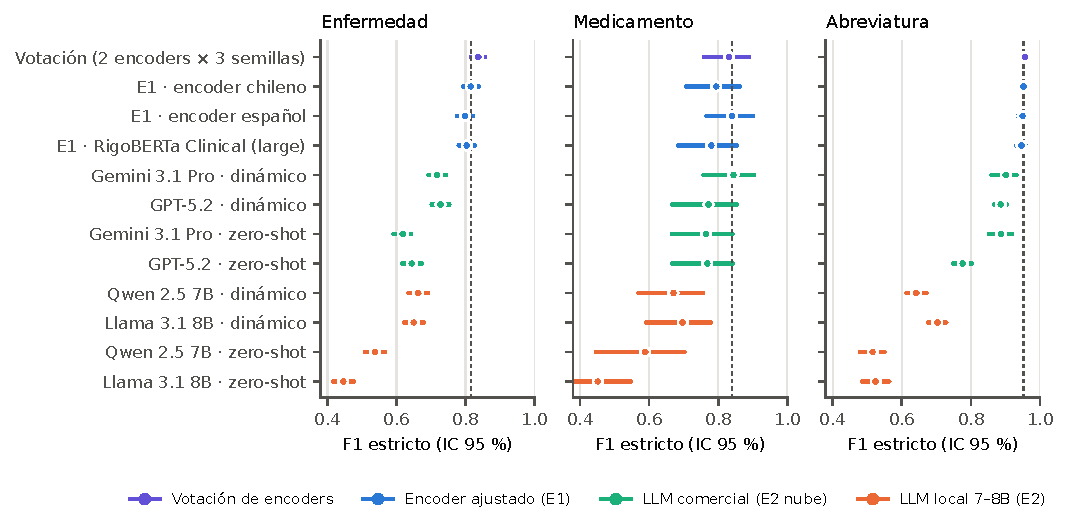
\includegraphics[width=0.95\textwidth]{figuras/fig_comparacion_f1.pdf}
\caption{F1 estricto con IC 95\,\% en las 990 oraciones de prueba. Para los encoders se muestra la media de tres semillas y el promedio de sus intervalos. La línea punteada marca el mejor encoder individual. La votación combina seis encoders base con mayoría estricta.}
\label{fig:comparacion}
\end{figure*}

\begin{table}[!t]
\centering
\caption{F1 estricto en el test (media $\pm$ DE de 3 semillas para E1). En negrita, el mayor valor de cada columna entre los sistemas individuales}
\label{tab:resultados}
\setlength{\tabcolsep}{3pt}
\begin{tabular}{lccc}
\toprule
Sistema & Enfermedad & Medicamento & Abreviatura \\
\midrule
E1 español & 0,798 $\pm$ 0,006 & 0,840 $\pm$ 0,012 & 0,950 $\pm$ 0,004 \\
E1 chileno & \textbf{0,815} $\pm$ 0,010 & 0,794 $\pm$ 0,046 & \textbf{0,952} $\pm$ 0,002 \\
E1 RigoBERTa & 0,803 $\pm$ 0,004 & 0,780 $\pm$ 0,015 & 0,946 $\pm$ 0,013 \\
\midrule
Llama 8B zero-shot & 0,446 & 0,451 & 0,524 \\
Llama 8B fijo & 0,526 & 0,393 & 0,603 \\
Llama 8B dinámico & 0,650 & 0,697 & 0,703 \\
Qwen 7B zero-shot & 0,537 & 0,589 & 0,516 \\
Qwen 7B fijo & 0,560 & 0,617 & 0,554 \\
Qwen 7B dinámico & 0,663 & 0,670 & 0,642 \\
\midrule
GPT-5.2 zero-shot & 0,645 & 0,768 & 0,776 \\
GPT-5.2 dinámico & 0,727 & 0,772 & 0,887 \\
Gemini 3.1 zero-shot & 0,618 & 0,765 & 0,888 \\
Gemini 3.1 dinámico & 0,717 & \textbf{0,844} & 0,901 \\
\midrule
E4 \emph{silver} + 50 \emph{gold} & 0,644 & 0,406$^\dagger$ & 0,592 \\
E4 \emph{silver} + 100 \emph{gold} & 0,650 & 0,674 & 0,634 \\
\midrule
Votación (6 encoders) & 0,837 & 0,831 & 0,957 \\
\bottomrule
\multicolumn{4}{l}{\footnotesize $^\dagger$Una de las tres semillas colapsó y no marcó ninguna entidad (Sec.~\ref{sec:e4}).}
\end{tabular}
\end{table}

Estos encoders superan a los del piloto del CWLC, que usó una versión más chica del corpus y obtuvo 0,77 en enfermedad, 0,75 en medicamento y 0,92 en abreviatura \cite{baez2020}. El mejor resultado publicado con el CWLC, 83,16 de micro-F1 sobre siete tipos de entidad \cite{rojas2022louhi}, usa otra partición y otras entidades, por lo que no se puede comparar directo.

En enfermedad, el encoder chileno superó al español por 2,6 y 2,4 puntos en dos semillas, con diferencias significativas, y por 0,2 en la tercera. Con nuestra regla de exigir las tres semillas no podemos afirmar que sea mejor, aunque la tendencia va siempre en la misma dirección. En medicamento rindió más el español. Ahí el chileno tuvo una corrida inestable (0,741 con la semilla 42) y la diferencia solo fue significativa en esa semilla. El test trae 92 medicamentos, y con tan pocas menciones los intervalos llegan a $\pm$7 puntos.

\subsection{LLM: el efecto de la estrategia}

Sin ejemplos, los LLM locales quedaron lejos, entre 0,45 y 0,59 de F1 estricto. Llama 3.1 8B en \emph{zero-shot} inventó el 52,5\,\% de las menciones que devolvió y entregó 22 JSON inválidos. Los ejemplos dinámicos mejoraron a los cuatro LLM en las tres entidades (Fig.~\ref{fig:estrategias}), lo que apoya H2. Frente a los ejemplos fijos, el \emph{few-shot} dinámico sumó 12,4 puntos en enfermedad y 10,0 en abreviatura con Llama, y 10,3 y 8,8 con Qwen, todos significativos. Es lo que reporta la literatura (5 a 9 puntos) o un poco más \cite{ge2026}. Sin las oraciones repetidas, la ventaja en enfermedad casi no cambió (12,4 puntos en Llama y 9,8 en Qwen), así que no viene de copiar oraciones idénticas.

\begin{figure*}[!t]
\centering
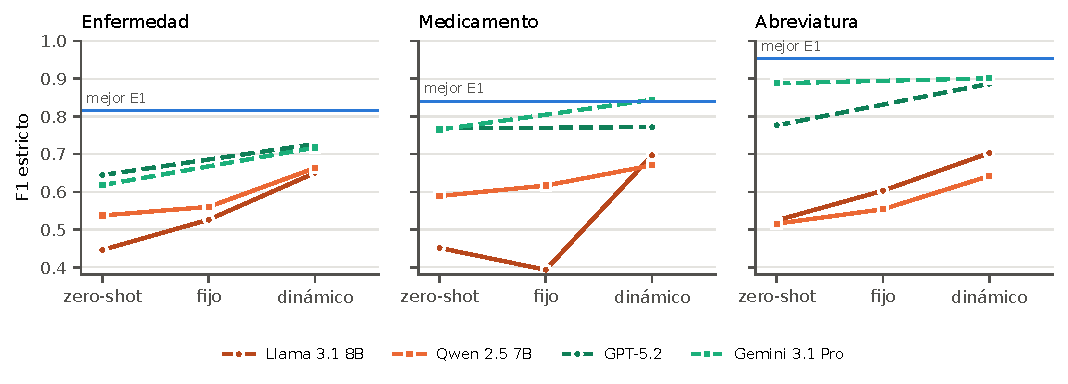
\includegraphics[width=0.95\textwidth]{figuras/fig_estrategias_llm.pdf}
\caption{F1 estricto de cada LLM según la estrategia de prompting. Para el \emph{few-shot} fijo se muestra la media de tres sets de ejemplos; a los LLM comerciales no se les aplicó esa estrategia. La línea azul marca el mejor encoder de E1 en cada entidad.}
\label{fig:estrategias}
\end{figure*}

Con su mejor estrategia, el mejor LLM local quedó entre 13,5 y 15,2 puntos bajo los encoders en enfermedad, 14,3 bajo el encoder español en medicamento y entre 24,7 y 24,9 en abreviatura. Todas estas diferencias fueron significativas contra cada semilla de E1. En enfermedad, la distancia está en el extremo alto de lo reportado en español \cite{naguib2024}. El problema de los LLM locales fue la precisión. Qwen con ejemplos dinámicos encontró el 71\,\% de las enfermedades, pero solo el 62\,\% de lo que marcó era correcto. Su F1 laxo en enfermedad (0,793) quedó 13 puntos sobre el estricto, contra 10 puntos en los encoders. Qwen fue más confiable que Llama: con ejemplos dinámicos inventó el 5,2\,\% de las menciones (Llama, el 19,4\,\%) y no entregó ningún JSON inválido.

Los LLM comerciales achicaron la distancia, pero solo la cerraron en una de las tres entidades. Esto apoya H5 en forma parcial. GPT-5.2 con ejemplos dinámicos llegó a 0,727 en enfermedad y 0,887 en abreviatura, y casi no inventó menciones (0,4\,\%). Gemini 3.1 Pro llegó a 0,717 y 0,901, y empató con el encoder en medicamento (0,844 contra 0,840 del encoder español, sin diferencia significativa). En medicamento, Gemini superó a GPT-5.2 por 0,073 (IC 95\,\% de 0,027 a 0,135); en las otras dos entidades no hubo diferencias significativas entre ambos. Contra E1, Gemini quedó entre 7 y 11 puntos abajo en enfermedad y entre 4 y 5 en abreviatura, con diferencias significativas en las tres semillas. Su recall en enfermedad (0,839) fue el más alto entre los LLM y quedó a la par del encoder chileno (0,836 de media), pero su precisión fue de 0,626 y su tasa de alucinación, de 14\,\%.

Con los modelos comerciales los ejemplos dinámicos también ayudaron: GPT-5.2 subió 8 puntos en enfermedad y 11 en abreviatura. Correr las 990 oraciones con ambas estrategias costó 4,26 dólares con GPT-5.2 y 4,46 con Gemini (Tabla~\ref{tab:costos}).

\begin{table}[!t]
\centering
\caption{Confiabilidad y costo de los LLM con \emph{few-shot} din\'amico}
\label{tab:costos}
\setlength{\tabcolsep}{3pt}
\small
\begin{tabular}{lcccc}
\toprule
Modelo & Alucin. & JSON inv. & s/oración & USD \\
\midrule
Llama 3.1 8B (local) & 19,4\,\% & 3 & 2,1 & 0 \\
Qwen 2.5 7B (local) & 5,2\,\% & 0 & 1,6 & 0 \\
GPT-5.2 (API) & 0,4\,\% & 0 & 2,0 & 2,52 \\
Gemini 3.1 Pro (API) & 14,2\,\% & 3 & 4,2 & 2,54 \\
\bottomrule
\multicolumn{5}{l}{\footnotesize Alucin.: menciones devueltas que no aparecen en la oración.}\\
\multicolumn{5}{l}{\footnotesize USD: costo de las 990 oraciones.}\\
\multicolumn{5}{l}{\footnotesize Tiempos locales en un Mac M5 de 24 GB.}
\end{tabular}
\end{table}

\subsection{Abreviaturas (H3)}

Los LLM reconocieron peor las enfermedades escritas con abreviatura. Con ejemplos dinámicos, el recall en enfermedades con y sin abreviatura fue 0,655 y 0,764 en Llama, 0,647 y 0,723 en Qwen, 0,748 y 0,804 en GPT-5.2, y 0,824 y 0,841 en Gemini. El encoder chileno no tuvo esa brecha (0,843 y 0,835). El español sí, aunque más chica (0,790 y 0,816). H3 se cumple en enfermedad. Este es el resultado que más apoya la adaptación al texto local: en enfermedades abreviadas, el encoder chileno superó al español por 5,3 puntos ($n=119$).

En la entidad abreviatura, la distancia entre LLM locales y encoders fue la mayor del estudio, de 25 a 31 puntos. Los LLM no aprendieron por sí solos las convenciones del corpus, como anotar ``APS'' o ``+'' como abreviaturas. Los comerciales las tomaron mejor de los ejemplos dinámicos y quedaron a 5 o 6 puntos.

\subsection{Escala del encoder}

RigoBERTa Clinical tiene 4,5 veces más parámetros que los encoders base y se preentrenó con el corpus clínico abierto más grande en español \cite{subies2025}. Aun así, no los superó en ninguna entidad. En enfermedad empató con el encoder español (diferencias de +0,003 a +0,008, ninguna significativa) y perdió contra el chileno en dos de tres semillas ($-0,018$ y $-0,019$). En medicamento quedó bajo el español en las tres semillas, con diferencia significativa en una. En abreviatura empató, salvo con la semilla 42. En este corpus importó más que el modelo hubiera visto derivaciones chilenas que su tamaño.

La excepción fueron las 66 abreviaturas que nunca aparecen en entrenamiento. Ahí RigoBERTa tuvo un recall de 0,662, contra 0,601 del encoder chileno y 0,606 del español. Tiene sentido para un modelo con un preentrenamiento clínico más amplio, aunque el subgrupo es chico. Hay también un costo práctico: el modelo \emph{large} no se pudo ajustar en el computador del proyecto y necesitó una GPU de 80 GB.

\subsection{Destilación con un LLM anotador (H4)}\label{sec:e4}

La Fig.~\ref{fig:e4} muestra la curva de E4. En enfermedad y abreviatura, el alumno superó a su maestro: con 50 oraciones \emph{gold}, el encoder entrenado con las etiquetas de Qwen llegó a 0,644 en enfermedad, y esas mismas etiquetas tenían 0,586. Las etiquetas \emph{silver} ayudaron cuando había poco \emph{gold}. Con 10 oraciones anotadas, el alumno llegó a 0,571 en enfermedad, y el modelo entrenado solo con esas 10 oraciones, a 0,278. Entre 50 y 100 oraciones la curva se aplanó (de 0,644 a 0,650).

\begin{figure*}[!t]
\centering
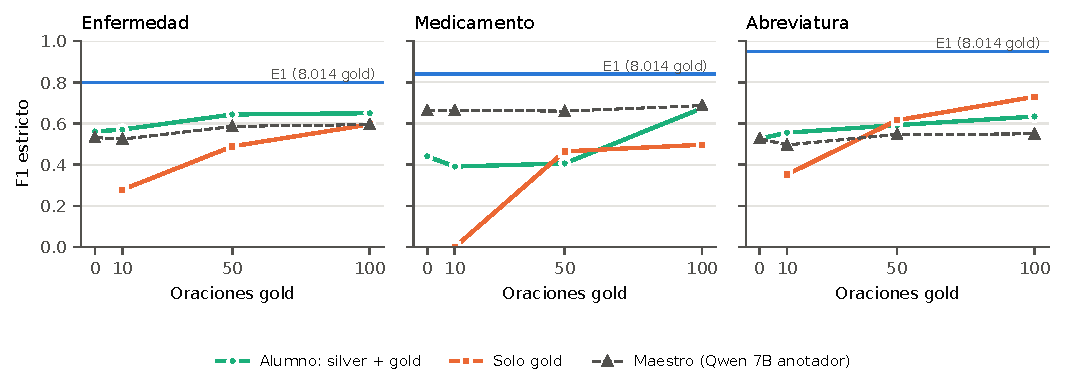
\includegraphics[width=0.95\textwidth]{figuras/fig_destilacion_e4.pdf}
\caption{Destilación (E4): F1 estricto medio de tres semillas según las oraciones \emph{gold} disponibles. El maestro es Qwen 2.5 7B; su F1 se mide contra el \emph{gold} de las 2.000 oraciones que etiquetó. En medicamento, con $N=0$, 10 y 50, una semilla del alumno colapsó y no marcó ninguna entidad; la media incluye esa semilla. El modelo entrenado solo con 10 oraciones \emph{gold} de medicamento obtuvo F1 0 en las tres semillas.}
\label{fig:e4}
\end{figure*}

H4 no se cumplió. Con 50 oraciones \emph{gold}, el alumno quedó entre 15 y 17 puntos bajo E1 en enfermedad, 23 en medicamento (con las dos semillas que no colapsaron) y 36 en abreviatura. En abreviatura, las etiquetas \emph{silver} incluso empeoraron el resultado: con 100 oraciones, entrenar solo con \emph{gold} dio 0,729, y agregar \emph{silver} lo bajó a 0,634. En esa entidad el maestro tuvo precisión alta (0,90) y recall bajo (0,49), porque no conocía las convenciones del corpus, y el alumno heredó ese sesgo. El F1 del maestro local fue de 0,50 a 0,69 según la entidad, y ese fue el techo del alumno.

En medicamento, una semilla colapsó: F1 0 y la pérdida estancada. Es la inestabilidad del ajuste fino en clases poco frecuentes que describen Dodge et al. y Mosbach et al. \cite{dodge2020,mosbach2021}. La reportamos tal cual, sin repetir la corrida con otra semilla.

E4 sí deja un dato útil. Con 100 oraciones anotadas, el alumno llegó en enfermedad a 0,650, casi lo mismo que el LLM local con ejemplos dinámicos (0,663). Ese LLM, en cambio, necesita las 8.014 oraciones de entrenamiento para buscar ejemplos y tarda más de un segundo por oración.

\subsection{Análisis de errores}

\begin{figure}[!t]
\centering
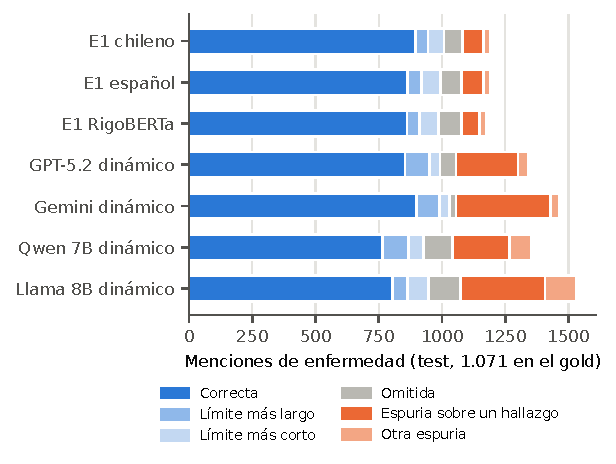
\includegraphics[width=\columnwidth]{figuras/fig_tipologia_errores.pdf}
\caption{Tipolog\'ia de predicciones de enfermedad en el test (semilla 42 para E1). ``Espuria sobre un hallazgo'': predicción que no coincide con ninguna enfermedad del \emph{gold} y que se superpone con un hallazgo (\ent{Finding}) anotado.}
\label{fig:tipologia}
\end{figure}

Con ejemplos dinámicos, los LLM comerciales acertaron casi tantas enfermedades exactas como el encoder: 899 Gemini y 854 GPT-5.2, contra 895 del encoder chileno (Fig.~\ref{fig:tipologia}). La diferencia de F1 estuvo en las predicciones espurias: 112 del encoder chileno, 286 de GPT-5.2, 406 de Gemini con ejemplos y 636 de Gemini sin ellos. Según el sistema, entre el 67\,\% y el 93\,\% de las espurias se superpuso con un hallazgo anotado, como ``dolor'', ``vómitos'' o ``mordida invertida''. La guía del CWLC separa el hallazgo (un signo o síntoma) de la enfermedad, y los LLM no siguieron esa separación aunque la guía estaba en el prompt. Parte del ``error'' de los LLM es un desacuerdo de criterio con la anotación.

\begin{figure}[!t]
\centering
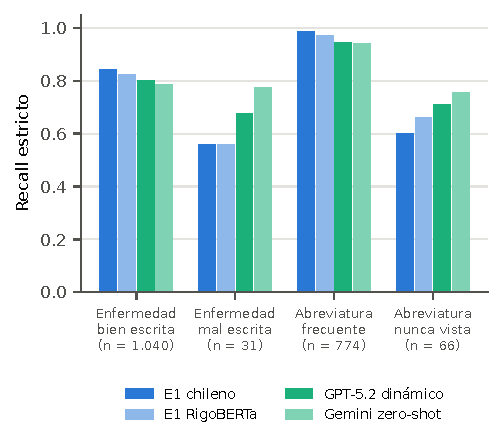
\includegraphics[width=\columnwidth]{figuras/fig_subgrupos_recall.pdf}
\caption{Recall estricto por subgrupo. Encoders: media de tres semillas. Las palabras mal escritas se detectaron con diccionario y distancia de edición y se revisaron a mano.}
\label{fig:subgrupos}
\end{figure}

En dos subgrupos, los LLM comerciales fueron mejores (Fig.~\ref{fig:subgrupos}). En las 31 enfermedades mal escritas, el recall de los encoders bajó de 0,82 o 0,84 a entre 0,52 y 0,56, mientras Gemini sin ejemplos se mantuvo en 0,77. En esas 31 menciones, la diferencia pareada entre Gemini y los encoders base fue de +0,19 a +0,32. Fue significativa en tres de las seis comparaciones (dos encoders por tres semillas); en las otras tres, el límite inferior del intervalo quedó en cero. La tokenización ayuda a entenderlo. Para el encoder, ``furosemida'' es una sola pieza, y ``FUSROSEMIDA'' son cinco que nunca vio juntas en entrenamiento \cite{moradi2021}. En las 66 abreviaturas nunca vistas, los encoders base llegaron a 0,60, y los LLM comerciales, a entre 0,71 y 0,76 (con ejemplos dinámicos, y Gemini también sin ellos; GPT-5.2 sin ejemplos llegó a 0,67). En las 774 abreviaturas frecuentes, los encoders llegaron a entre 0,97 y 0,99. El encoder reconoce casi siempre la jerga que vio en entrenamiento; la que no vio, los LLM grandes la deducen mejor. Los LLM locales no tuvieron esa ventaja: en enfermedades nuevas, su recall (0,56 a 0,60) quedó bajo el de los encoders (0,70 a 0,73).

Como cada tipo de modelo acierta en casos distintos, probamos combinarlos. Si se juntan las enfermedades que encuentra el encoder con las que encuentra un LLM, el recall llega a entre 0,87 y 0,92; el del encoder solo está entre 0,81 y 0,84. Probamos tres combinaciones simples: la unión de ambas predicciones, agregar solo las del LLM que no chocan con las del encoder, y agregar solo las que caen en palabras que el encoder nunca vio. Las tres empeoraron el F1 en enfermedad de forma significativa, porque cada acierto del LLM llega con varios falsos positivos. Un híbrido útil necesitaría usar la confianza del encoder o un paso de verificación, y lo dejamos como trabajo futuro. Por ahora, las palabras mal escritas son el 3\,\% de las enfermedades del test y no justifican un componente aparte.

\subsection{Votación entre encoders}

Combinar semillas rindió más que agrandar el modelo. La votación de los seis encoders base llegó a 0,837 en enfermedad (IC 95\,\% de 0,815 a 0,857), con precisión de 0,862 y recall de 0,813. Superó a cada uno de los seis modelos por separado, por 1,3 a 4,5 puntos y con diferencias significativas. Es el mejor resultado del estudio en esa entidad. En abreviatura llegó a 0,957, mejor que dos de los seis modelos, y en medicamento a 0,831, sin diferencias significativas. Con las tres semillas de RigoBERTa (nueve modelos y cinco votos), el F1 de enfermedad quedó en 0,838, y ya no fue significativamente mejor que todos los modelos individuales. La ganancia de la votación sale de promediar la variación entre semillas de los dos encoders base. El costo es correr seis modelos de 125M en vez de uno, algo que un computador común todavía puede hacer.

\subsection{Resumen de hipótesis}

La Tabla~\ref{tab:hipotesis} resume las hipótesis. En las derivaciones chilenas se repitió lo que reporta la literatura: el encoder ajustado gana y los ejemplos dinámicos ayudan. Hubo dos sorpresas. La destilación quedó mucho más lejos del encoder de lo esperado, y un LLM comercial empató con el encoder en medicamento.

\begin{table}[!t]
\centering
\caption{Resultado de las hip\'otesis}
\label{tab:hipotesis}
\begin{tabular}{p{0.6cm}p{2.0cm}p{4.9cm}}
\toprule
 & Resultado & Evidencia \\
\midrule
H1 & Apoyada & Mayor F1 en enfermedad y abreviatura; en medicamento, empate con Gemini dinámico \\
H2 & Apoyada & Dinámico $>$ \emph{zero-shot} en los cuatro LLM y $>$ fijo en los dos locales \\
H3 & Apoyada en enfermedad & Con ejemplos dinámicos, los cuatro LLM tienen menor recall en enfermedades abreviadas; el encoder chileno no tiene brecha \\
H4 & No apoyada & Con 50 \emph{gold}, 15 a 36 puntos bajo E1 \\
H5 & Apoyada en 2 de 3 & Los LLM comerciales quedan bajo E1 en enfermedad y abreviatura; Gemini empata en medicamento \\
\bottomrule
\end{tabular}
\end{table}

\subsection{Limitaciones}\label{sec:limitaciones}

Una derivación es un texto corto, escrito para justificar una interconsulta, y los resultados podrían cambiar en las evoluciones o los planes de cuidado de una ficha de CESFAM. Hoy no existe en Chile un corpus público de ese tipo.

También hay riesgo de contaminación. El encoder chileno se preentrenó con derivaciones de la lista de espera, sin que se publique cuáles, y pudo haber visto oraciones del test. Los LLM comerciales pudieron ver el CWLC, que es público desde 2022. Si eso pasó, sus resultados son un techo optimista.

El corpus tiene ruido de anotación (42 textos idénticos anotados de forma distinta), y medicamento tiene solo 92 menciones en el test, con intervalos de $\pm$7 puntos. Corrimos los LLM una vez por estrategia. Con temperatura 0 la variación debería ser baja, pero no la medimos, y Gemini estaba en versión preliminar durante los días de la corrida. Por tiempo, no evaluamos el ajuste fino de un LLM con LoRA (E3) ni la normalización previa de abreviaturas (E5). Por último, la distinción entre ``hallazgo'' y ``enfermedad'' de la guía del CWLC penaliza a los LLM, y con otra guía esa parte del resultado podría cambiar.

%==============================================================================
\section{Conclusiones}\label{sec:conclusiones}
%==============================================================================

Con derivaciones reales de APS chilena se repitió lo que reporta la literatura internacional: un encoder ajustado con datos anotados reconoce enfermedades, medicamentos y abreviaturas mejor que un LLM generativo con prompting. El encoder adaptado a derivaciones chilenas tuvo el mejor F1 individual en enfermedad (0,815), y la votación de seis encoders base subió esa cifra a 0,837. Un encoder 4,5 veces más grande no mejoró el resultado. Los ejemplos recuperados por similitud mejoraron a todos los LLM, pero los locales de 7 y 8B siguieron entre 13 y 25 puntos abajo, y la destilación con 50 oraciones anotadas quedó lejos del encoder.

Los LLM comerciales reconocieron mejor que el encoder las palabras mal escritas y las abreviaturas que nunca aparecieron en entrenamiento. A cambio, marcaron muchos hallazgos como enfermedades, y para usarlos hay que enviar el texto a un servicio externo.

Para un CESFAM, la recomendación es concreta. Si tiene texto anotado, la opción más precisa es un encoder base ajustado con texto local, o una votación de varios: corre en un computador común y no saca datos del centro. Si no lo tiene, le conviene anotar algunos cientos de oraciones con criterio clínico antes que confiar en etiquetas generadas por un LLM local.

\subsection*{Trabajo futuro}

Queda trabajo pendiente en tres líneas. Una es un sistema híbrido que use la confianza del encoder para decidir cuándo consultar al LLM. Otra es validar los modelos en evoluciones y planes de cuidado de CESFAM, que es el objetivo de la tesis doctoral del primer autor. La última es medir qué pasa con texto escrito por pacientes, con lenguaje coloquial y ruido de mensajería; para eso ya armamos una lista de equivalencias, que falta revisar con clínicos.

\section*{Disponibilidad de c\'odigo y datos}
El código, los prompts, las configuraciones y los resultados están en \url{https://github.com/SebasDCIS/proyecto-ner-aps-genai}. El CWLC está disponible en Zenodo (registro 5591011) bajo licencia CC BY-NC-SA 4.0.

\section*{Agradecimientos}
Se usaron herramientas de IA como apoyo en la programación y la edición del texto.

\bibliographystyle{IEEEtran}
\bibliography{referencias}

\end{document}
